\chapter{Οι Αλγόριθμοι}
\label{ch:Algorithms}

Σε αυτό το κεφάλαιο θα μελετήσουμε με λεπτομέρεια όλους τους αλγορίθμους που υλοποιήσαμε για τα AT-free γραφήματα.
Για κάθε αλγόριθμο θα δώσουμε τον συμβολισμό και τα λήμματα που χρειάζονται για την περιγραφή του. Αμέσως μετά, θα εξηγήσουμε την πολυπλοκότητά του και συγκεκριμένα βήματά του, που θεωρήσαμε πιο ιδιαίτερα. Τέλος θα δώσουμε και ένα απλό παράδειγμα επίλυσης του κάθε αλγορίθμου.

Διευκρινίζουμε ότι δεν αποδεικνύουμε την ορθότητα του κάθε αλγορίθμου που χρησιμοποιούμε. Οι αποδείξεις αυτές βρίσκονται στις αντίστοιχες αναφορές(\cite{at-free-independent-sets}, \cite{at-free-domination}, \cite{at-free-3-colouring})   

% -------------
% SECTION START
% -------------
\section{Υπολογισμός Μέγιστου Ανεξάρτητου Συνόλου}
\label{sec:Independent_Set_Alg}
Συμβολίζουμε τον αριθμό των κορυφών ενός γραφήματος $G = (V, E)$ με
$n$ και τον αριθμό των ακμών με $m$. 
Υπενθυμίζουμε ότι ένα ανεξάρτητο σύνολο σε ένα γράφημα $G$ είναι ένα σύνολο από ζεύγη με μη γειτονικές
κορυφές. Ο αριθμός ανεξαρτησίας ενός γραφήματος $G$, συμβολίζεται ως $\alpha(G)$ είναι το μέγεθος
του μεγαλύτερου ανεξάρτητου συνόλου στο γράφημα. Οι βασικές δομικές ιδιότητες που πρέπει να αναλύσουμε πριν την περιγραφή του αλγορίθμου είναι τα $Components$ και τα $Intervals$.


Σε ένα AT-free γράφημα $G$ όπου το $x$ και το $y$ είναι δύο ξεχωριστές μη γειτονικές κορυφές του G. Συμβολίζουμε με $C^{x}(y)$ το $Component$ του $G - N[x]$ όπου εμπεριέχεται το $y$, και με $r(x)$ τον αριθμό των $Components$ του $G - N[x]$.

\begin{definition}
	Μια κορυφή $z \in V \setminus \{x, y\}$ είναι μεταξύ των κορυφών $x$ και $y$ εάν οι $x$ και $z$ βρίσκονται στον ίδιο $Component$ του $G - N[x]$. Εναλλακτικά, η κορυφή $z$ είναι μεταξύ των $x$ και $y$ στο γράφημα $G$ αν υπάρχει μονοπάτι από τον $x$ στον $z$ που αποφεύγει το $N[y]$ και μονοπάτι από τον $y$ στον $z$ που αποφεύγει το $N[x]$.
\end{definition}

\begin{definition}
	Το διάστημα $I = I(x, y)$ του $G$ είναι το σύνολο όλων των κορυφών του $G$ που βρίσκονται μεταξύ $x$ και $y$. Συνεπώς, $I(x, y) = C_x(y) \cap C_y(x)$.
\end{definition}

 Ο αλγόριθμος των Broersma, H., Kloks, T., Kratsch, D. και Müller, H. του καθορίζει τον αριθμό ανεξαρτησίας κάθε $Component$ και κάθε $Interval$ χρησιμοποιώντας τις σχέσεις που δίνονται στα Λήμματα \ref{lemma6_1}, \ref{lemma6_2} και \ref{lemma6_3}.
 
 \begin{lemma}
 	\label{lemma6_1}
 	'Έστω ότι $G = (V,E)$ είναι οποιαδήποτε γράφημα. 
 	Τότε $$\alpha(G)=1+\max_{x\in V}\left(\sum_{i=1}^{r(x)}\alpha(C_i^x)\right)$$ όπου  $C_1^x, C_2^x,...,C_r(x)^x$ τα $Compontes$ του $G - N[x]$.
 \end{lemma}

\begin{lemma}
	\label{lemma6_2}
		'Έστω ότι $G = (V,E)$ είναι ένα AT-free γράφημα. Έστω $x \in V$ και έστω $C^x$ ένα $Component$ του $G - N[x]$. Τότε $$\alpha(C^x)=1+\max_{y\in C^x}\left(\alpha(I(x,y))+\sum_{i}\alpha(D_i^y)\right)$$ όπου τα $D_i^y$ είναι $Components$ του $G - N[y]$ που εμπεριέχονται στο $C^x$. 
\end{lemma}

\begin{lemma}
	\label{lemma6_3}
	'Έστω ότι $G = (V,E)$ είναι ένα AT-free γράφημα. Έστω $I = I(x,y)$ είναι ένα $Interval$ του $G$. Αν $I = \emptyset$ τότε $\alpha(I) = 0$. Αλλιώς $$\alpha(I)=1+\max_{s\in I}\left(\alpha(I(x,s))+\alpha(I(s,y))+\sum_{i}\alpha(C_i^s)\right)$$
\end{lemma}
	
Σε αυτό το σημείο μπορούμε να δώσουμε τον αλγόριθμο για τον υπολογισμό του αριθμού ανεξαρτησίας $\alpha(G)$ για AT-free γραφήματα, ο οποίος είναι βασισμένος στον δυναμικό προγραμματισμό. 

\begin{algorithm}[H]
	\caption{Αλγόριθμος υπολογισμού αριθμού ανεξαρτησίας σε AT-free γραφήματα}
	\label{alg:DOPC}
	
	\hspace*{\algorithmicindent} \textbf{Είσοδος:} Ένα AT-free γράφημα $G$.\\
	 
	\hspace*{\algorithmicindent} \textbf{Έξοδος:} Αριθμός ανεξαρτησίας $\alpha(G)$
	
	\begin{algorithmic}[1]
		
		\STATE Για κάθε $x \in V$, υπολόγισε όλα τα $Components$ $C_1^x , C_2^x , \ldots , C_{r(x)}^x$
		\STATE Για κάθε ζευγάρι μη γειτονικών κορυφών $x$ και $y$, υπολόγισε το $Interval$ $I(x, y)$.
		\STATE Ταξινόμησε όλα τα $Components$ και τα $Intervals$ με βάση το μη-αύξοντα αριθμό κορυφών.
		\STATE Υπολόγισε τα $\alpha(C)$ και $\alpha(I)$ για κάθε $Components$ $C$ και κάθε $Interval$ $I$ με τη σειρά του Βήματος 3.
		\STATE Υπολόγισε το $\alpha(G)$.
				
	\end{algorithmic}
\end{algorithm}

\begin{definition}
	 Υπάρχει αλγόριθμος χρόνου $O(n^4)$ για τον υπολογισμό του ανεξάρτητου αριθμού ενός AT-free γραφήματος.
\end{definition}

Για την πολυπλοκότητα του αλγορίθμου μελετάμε κάθε βήμα ξεχωριστά. Το πρώτο βήμα μπορεί να υλοποιηθεί σε χρόνο $O(n(n + m))$ χρησιμοποιώντας έναν γραμμικό αλγόριθμο για τον υπολογισμό των $Components$. 

Το βήμα 2 υπολογίζει $Intervals$ για τις μη γειτονικές κορυφές $x$ και $y$, χρησιμοποιώντας την τομή των συνιστωσών $C_x(y)$ και $C_y(x)$. Η διαδικασία, που εκτελείται σε χρόνο O(n) για κάθε $Interval$, οδηγεί σε συνολική χρονική πολυπλοκότητα $O(n^3)$. Η υλοποίηση αξιοποιεί ένα λεξικό με αντικείμενα της κλάσης $Interval$, παρέχοντας έναν αποτελεσματικό τρόπο διαχείρισης και υπολογισμού εντός το πολύ $n^2$ $Component$ και $Intervals$.

Με την χρήση του Bucket sort το βήμα 3 υλοποιείται σε $O(n^2)$.

Το σημείο φραγμού για τη χρονική πολυπλοκότητα του αλγορίθμου μας είναι το βήμα 4 αφού εκτελείται σε $O(n^4)$. Για κάθε $Component$ $C_x$ του $G - N[x]$ και μια κορυφή $y \in C_x$, ο αλγόριθμος πρέπει να υπολογίσει τα $Components$ του $G - N[y]$ που περιέχονται στην $C_x$. Αυτό γίνεται σε χρόνο $O(|C_x|)$ για σταθερές κορυφές $x$ και $y$ στο $C_x$, με αποτέλεσμα ο συνολικός χρόνος να είναι $O(n^3)$ για όλα τα $Compoents$. Θεωρώντας ένα $Interval$ $I(x, y)$ και μια κορυφή $s \in I$, ο αλγόριθμος πρέπει να αθροίσει τους αριθμούς ανεξαρτησίας των $Components$ $C_s$ του $G - N[s]$ που περιέχονται στο $I$. Η λειτουργία αυτή απαιτεί χρόνο $O(|I(x, y)|)$ για ένα σταθερό $I(x, y)$ και μια κορυφή $s \in I$. Ο συνολικός χρόνος για τον υπολογισμό του $\alpha(I)$ για όλα τα διαστήματα είναι $O(n^3)$.

Είναι σαφές ότι το βήμα 5 μπορεί να γίνει σε χρόνο $O(n^2)$. Έτσι ο χρόνος εκτέλεσης του αλγορίθμου μας
είναι $O(n^4)$.

Παρακάτω παραθέτουμε ένα παράδειγμα εκτέλεσης του αλγορίθμου για το γράφημα \ref{fig:at-free-graph-example}.

\begin{figure}[H]
	\centering
	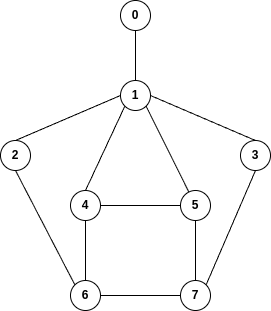
\includegraphics[width=0.4\textwidth]{pictures/at-free-graph.png} 
	\caption{Ένα AT-free γράφημα με 7 κόμβους}
	\label{fig:at-free-graph-example}
\end{figure}

Μετά την εκτέλεση του πρώτου βήματος τα $Components$ που υπολογίσαμε φαίνονται στον πίνακα \ref{table:first-step-intependent-set} 

% Components
\begin{table}[H]
	
	\centering
	\caption{Components του γραφήματος μετά την εκτέλεση του πρώτου βήματος}
	\begin{tabular}{|c|c|c|}
		\hline
		\textbf{Component} & \textbf{Σύνολο κορυφών} & \textbf{Alpha} \\
		\hline
		$C_1^2$ & \quad \{3, 4, 5, 7\} & - \\
		$C_2^2$ & \quad \{0\} & - \\
		$C_1^5$ & \quad \{2, 3, 4, 6\} & - \\
		$C_2^5$ & \quad \{0\} & - \\
		$C_1^1$ & \quad \{6, 7\} & - \\
		$C_1^0$ & \quad \{2, 3, 4, 5, 6, 7\} & - \\
		$C_1^4$ & \quad \{2, 6\} & - \\
		$C_2^4$ & \quad \{5\} & - \\
		$C_3^4$ & \quad \{0\} & - \\
		$C_1^7$ & \quad \{0, 1, 2, 3\} & - \\
		$C_1^3$ & \quad \{2\} & - \\
		$C_2^3$ & \quad \{5, 7\} & - \\
		$C_3^3$ & \quad \{0\} & - \\
		$C_1^6$ & \quad \{0, 1, 4, 5\} & - \\
		\hline
	\end{tabular}
\label{table:first-step-intependent-set}
\end{table}

Για το δεύτερο βήμα του αλγορίθμου, παίρνοντας όλους τους συνδυασμούς μη γειτονικών κορυφών για το παρών γράφημα. Τα $Intervals$ που προκύπτουν φαίνονται στον παρακάτω πίνακα\ref{table:second-step-intependent-set}. 

\begin{table}[H]
	
	\centering
	\caption{Intervals του γραφήματος μετά την εκτέλεση του δεύτερου βήματος}
	\begin{tabular}{|c|c|c|}
		\hline
		\textbf{Intervals} & \textbf{Σύνολο κορυφών} & \textbf{Alpha} \\
		\hline
		I(2, 5) & \quad \{3, 4\} & - \\
		I(2, 7) & \quad \{3\} & - \\
		I(5, 2) & \quad \{3, 4\} & - \\
		I(5, 6) & \quad \{4\} & - \\
		I(0, 7) & \quad \{2, 3\} & - \\
		I(0, 6) & \quad \{4, 5\} & - \\
		I(7, 2) & \quad \{3\} & - \\
		I(7, 0) & \quad \{2, 3\} & - \\
		I(6, 5) & \quad \{4\} & - \\
		I(6, 0) & \quad \{4, 5\} & - \\
		\hline
	\end{tabular}
\label{table:second-step-intependent-set}
\end{table}

Όπως φαίνεται και στους πίνακες \ref{table:sorted-components} και \ref{table:sorted-intervals},μετά το τρίτο βήμα τα $Components$ και $Intervals$ ταξινομούνται με βάση το πλήθος των κορυφών τους, από το μικρότερο στο μεγαλύτερο.

\begin{table}[H]
	\centering
	\caption{Ταξινόμηση Components με βάση το σύνολο κορυφών}
	\begin{tabular}{|c|c|c|}
		\hline
		\textbf{Components} & \textbf{Σύνολο Κορυφών} & \textbf{Alpha} \\
		\hline
		$C_2^2$ & \{0\} & - \\
		$C_2^5$ & \{0\} & - \\
		$C_3^4$ & \{0\} & - \\
		$C_3^3$ & \{0\} & - \\
		$C_2^4$ & \{5\} & - \\
		$C_1^7$ & \{0, 1, 2, 3\} & - \\
		$C_1^1$ & \{6, 7\} & - \\
		$C_1^4$ & \{2, 6\} & - \\
		$C_1^3$ & \{2\} & - \\
		$C_1^2$ & \{3, 4, 5, 7\} & - \\
		$C_1^5$ & \{2, 3, 4, 6\} & - \\
		$C_1^6$ & \{0, 1, 4, 5\} & - \\
		$C_1^0$ & \{2, 3, 4, 5, 6, 7\} & - \\
		\hline
	\end{tabular}
	\label{table:sorted-components}
\end{table} 

\begin{table}[H]
	\centering
	\caption{Ταξινόμηση Intervals με βάση το σύνολο κορυφών}
	\begin{tabular}{|c|c|c|}
		\hline
		\textbf{Intervals} & \textbf{Σύνολο Κορυφών} & \textbf{Alpha} \\
		\hline
		I(2, 7) & \{3\} & - \\
		I(5, 6) & \{4\} & - \\
		I(7, 2) & \{3\} & - \\
		I(6, 5) & \{4\} & - \\
		I(2, 5) & \{3, 4\} & - \\
		I(5, 2) & \{3, 4\} & - \\
		I(0, 7) & \{2, 3\} & - \\
		I(0, 6) & \{4, 5\} & - \\
		I(7, 0) & \{2, 3\} & - \\
		I(6, 0) & \{4, 5\} & - \\
		\hline
	\end{tabular}
	\label{table:sorted-intervals}
\end{table}

Χρησιμοποιώντας τα λήμματα \ref{lemma6_1}, \ref{lemma6_2} και εφαρμόζοντας τεχνικές δυναμικού προγραμματισμού, μετά την εκτέλεση του βήματος τέσσερα έχουν υπολογιστεί τα alpha όλων των $Components$ και $Intervals$. Τα αποτελέσματα φαίνονται στους πίνακες \ref{table:computed-alpha-componentes}  και \ref{table:computed-alpha-intervals}

\begin{table}[H]
	\centering
	\caption{Πίνακας Components μετά την εκτέλεση του βήματος 4 του αλγορίθμου}
	\begin{tabular}{|c|c|c|}
		\hline
		\textbf{Components} & \textbf{Σύνολο Κορυφών} & \textbf{Alpha} \\
		\hline
		$C_2^2$ & \{0\} & 1 \\
		$C_2^5$ & \{0\} & 1 \\
		$C_3^4$ & \{0\} & 1 \\
		$C_3^3$ & \{0\} & 1 \\
		$C_2^4$ & \{5\} & 1 \\
		$C_1^7$ & \{0, 1, 2, 3\} & 3 \\
		$C_1^1$ & \{6, 7\} & 1 \\
		$C_1^4$ & \{2, 6\} & 1 \\
		$C_1^3$ & \{2\} & 1 \\
		$C_1^2$ & \{3, 4, 5, 7\} & 2 \\
		$C_1^5$ & \{2, 3, 4, 6\} & 2 \\
		$C_1^6$ & \{0, 1, 4, 5\} & 3 \\
		$C_1^0$ & \{2, 3, 4, 5, 6, 7\} & 3 \\
		\hline
	\end{tabular}
	\label{table:computed-alpha-componentes}
\end{table} 

\begin{table}[H]
	\centering
	\caption{Πίνακας Intervals μετά την εκτέλεση του βήματος 4 του αλγορίθμου}
	\begin{tabular}{|c|c|c|}
		\hline
		\textbf{Intervals} & \textbf{Σύνολο Κορυφών} & \textbf{Alpha} \\
		\hline
		I(2, 7) & \{3\} & 1 \\
		I(5, 6) & \{4\} & 1 \\
		I(7, 2) & \{3\} & 1 \\
		I(6, 5) & \{4\} & 1 \\
		I(2, 5) & \{3, 4\} & 1 \\
		I(5, 2) & \{3, 4\} & 1 \\
		I(0, 7) & \{2, 3\} & 2 \\
		I(0, 6) & \{4, 5\} & 2 \\
		I(7, 0) & \{2, 3\} & 2 \\
		I(6, 0) & \{4, 5\} & 2 \\
		\hline
	\end{tabular}
	\label{table:computed-alpha-intervals}
\end{table}

Στο τελευταίο βήμα με την εφαρμογή του λήμματος \ref{lemma6_1}, είναι προφανές ότι ο αριθμός ανεξαρτησίας για το παρόν γράφημα είναι τέσσερα. Αυτό μπορεί, στο συγκεκριμένο παράδειγμα, να προκύψει από διάφορες κορυφές.



\section{Υπολογισμός Ελάχιστου Κυρίαρχου Συνόλου}
\label{sec:Domination_Set_Alg}


% SECTION START
% -------------
\section{Το Πρόβλημα του 3-Χρωματισμού}
\label{sec:3-Coloring_Alg}

 








